\chapter{Experimental evaluation for a simple problem}

Before moving on to a Multi-instance target propagation problem, the target propagation method was tested on a simple problem. The dataset used as such a "toy" problem is the \VUname{two-moon dataset}.

\section{The two-moon dataset}
The dataset consists of 2D spatial data. Each datum is a point in the \( \left( 0, 1 \right) \times \left( 0, 1 \right) \) space. The data is split into two classes, each forming a distinct shape of a crescent moon when plotted (see figure \ref{twomoon}). The two moons are inter-twinned, making the dataset not linearly separable. The actual dataset used was generated as follows:

The negative class was generated by drawing \( x \sim \mathcal{U} \left( 0.3, 0.9 \right) \) and calculating
\[ y = -2 \sqrt{0.3^2 - \left( x - 0.6 \right)^2} + 0.7 \]
This means the points lie on an ellipse with the center at \( \begin{pmatrix} 0.6 \\ 0.7 \end{pmatrix} \) and a semi-major and a semi-minor axis of \( 0.3 \) and \( 0.6 \), the same as for the negative class.

The positive class was generated by drawing \( x \sim \mathcal{U} \left( 0.1, 0.7 \right) \) and calculating
\[ y = 2 \sqrt{0.3^2 - \left( x - 0.4 \right)^2} + 0.3 \]
This means the points lie on an ellipse with the center at \( \begin{pmatrix} 0.4 \\ 0.3 \end{pmatrix} \) and a semi-major and a semi-minor axis of \( 0.3 \) and \( 0.6 \).

A random noise was added to both elements of all data points in both classes. The noise was drawn from \( \mathcal{N} \left(0, 0.025 \right) \).

\begin{graph}[h]
	\centering
	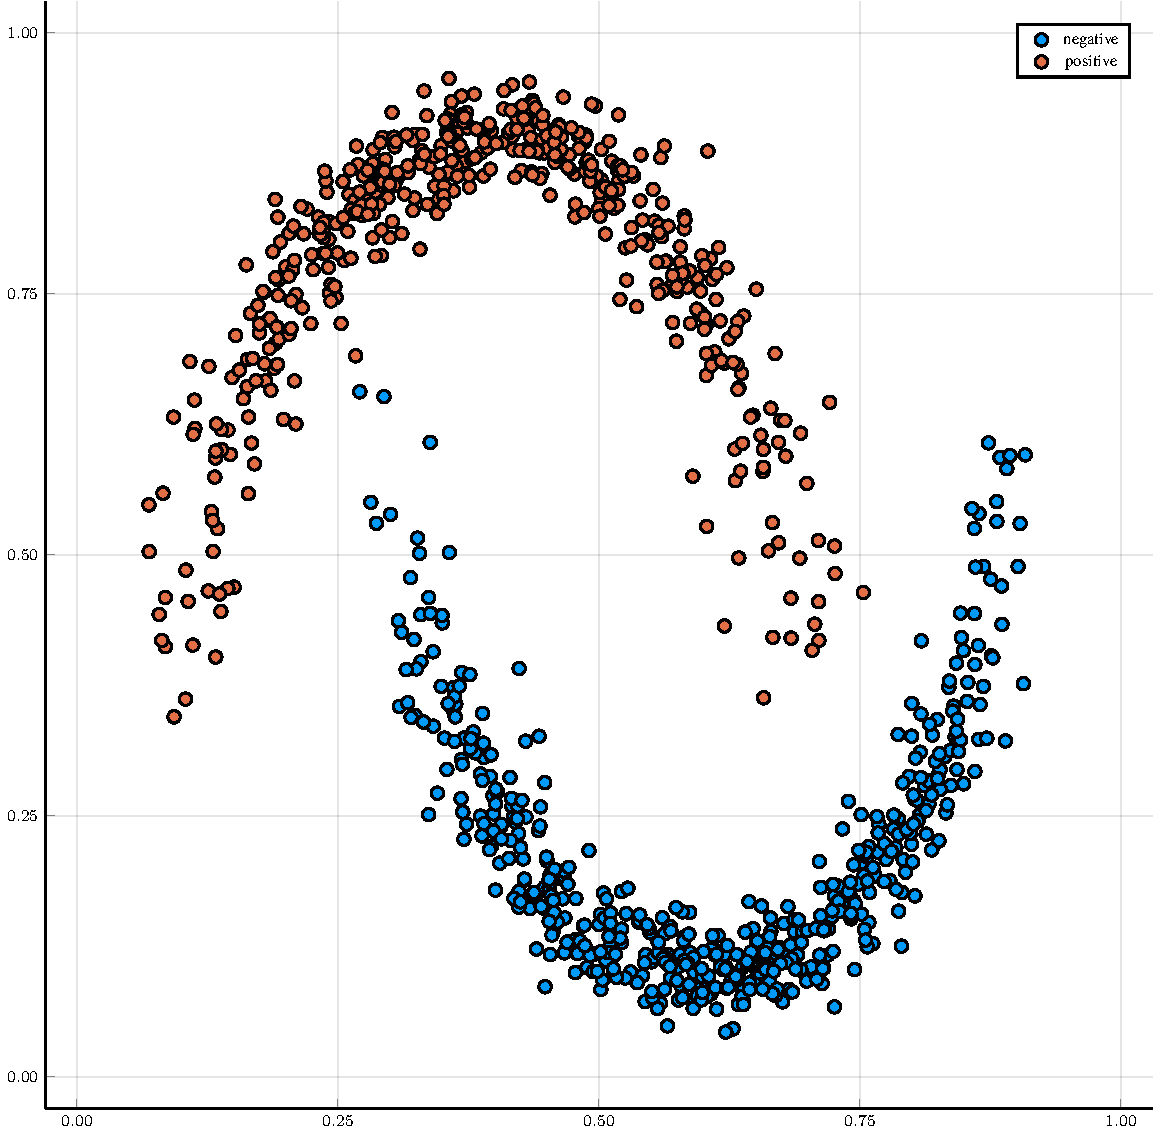
\includegraphics[width=\textwidth]{images/two-moon/two-moon.pdf}
	\caption{Example of a Two-moon dataset}\label{twomoon}
\end{graph}

\todo{Backprop on this DS}

\section{The used model}

The model used to classify these samples is a layer of 16 neurons, followed by a layer of 2 neurons, followed by the softmax function in order to represent the output as a measure of confidence that a given sample belongs to a given class. The activations used for the neurons were the tanh function, the ReLU function (see \cite{hahnloser_digital_2000}) and the swish function (see \cite{ramachandran_searching_2018}). ADAM (see \cite{kingma_adam:_2014}) was used as the optimisation method. The mean squared error function was used as the model loss as well as the layer-local loss function for all the layers. The training dataset consisted of a 1000 random samples, the testing dataset was 100 samples. The network was taught on the training dataset in 2000 epochs.

To learn the inverse mappings the same model was used for both of the first two layers. This model consisted of a layer of 8 neurons followed by a layer with as many neurons as was the required input dimension. The second of those used identity as an activation function, the first used the same activation as the rest of the network. The inverse mapping for the softmax function consisted of a layer of 4 neurons followed by a layer of 2 neurons with the identity function as its activation. The mean squared error function was used as the dual layer-local loss function for all the inverse mappings. The noise inserted for the auto-encoder training was \( \varepsilon \sim N \left( 0, 0.2 \right) \). The step size for the last layer target (see equation \ref{targetprop_last_layer_target}) was \( \eta = 0.5 \).

\section{Results}

The model was tested with 3 activation functions. See figures \ref{tanh}, \ref{relu}, \ref{swish}. \todo{Proper figures}

\begin{graph}[h]
	\centering
	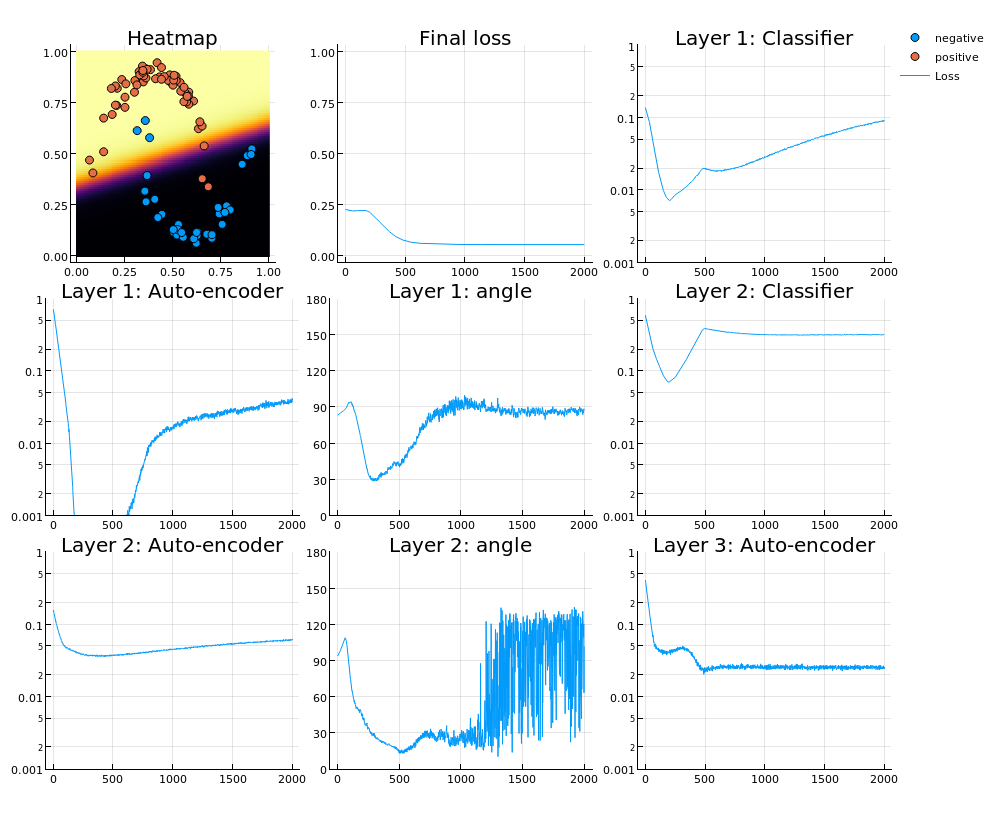
\includegraphics[width=\textwidth]{images/temp-tanh.png}
	\caption{Results with the tanh activation function}\label{tanh}
\end{graph}

\begin{graph}[h]
	\centering
	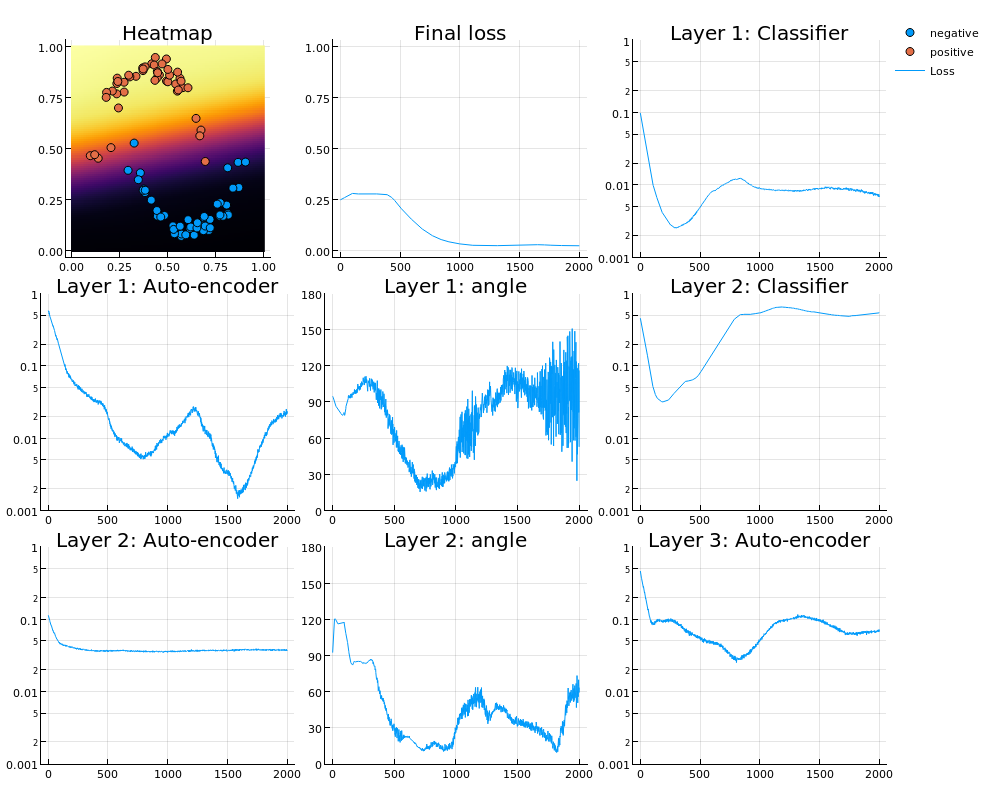
\includegraphics[width=\textwidth]{images/temp-relu.png}
	\caption{Results with the ReLU activation function}\label{relu}
\end{graph}

\begin{graph}[h]
	\centering
	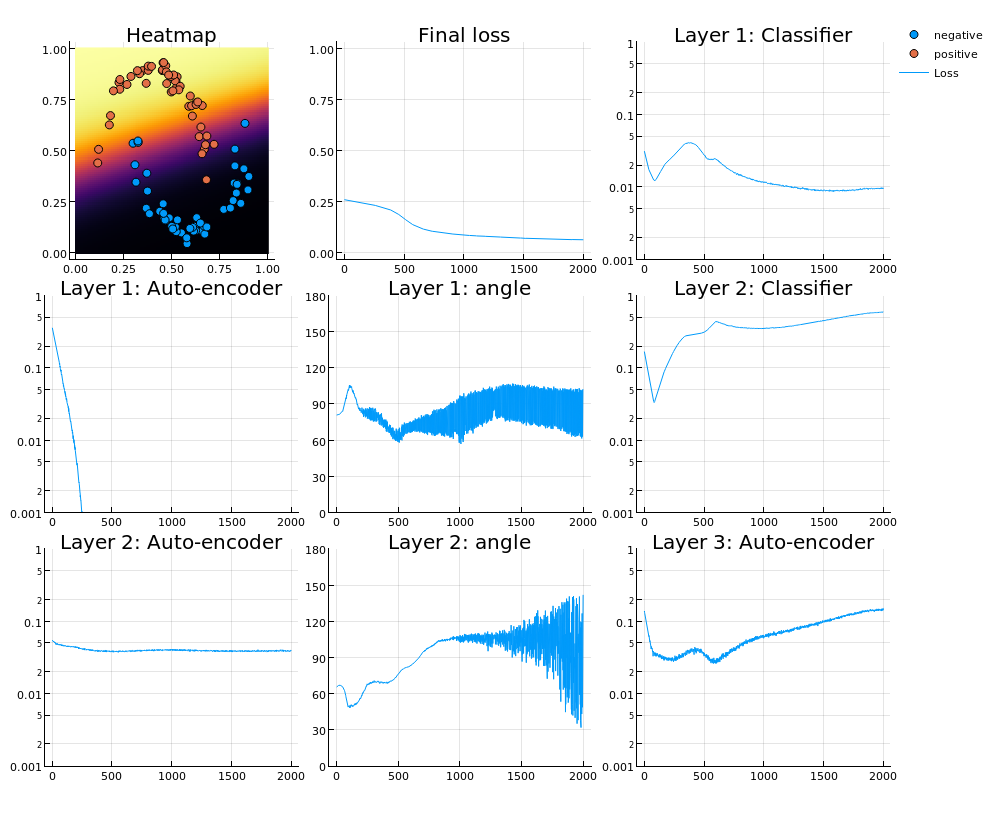
\includegraphics[width=\textwidth]{images/temp-swish.png}
	\caption{Results with the swish activation function}\label{swish}
\end{graph}

\section{Explanation of the results}

As can be seen from the results, the model fails to learn anything more than a simple linear separation. In this section, a possible explanation of this behaviour is proposed.

As a result of the architecture of a target-propagation model, the most crucial layer for the learning is the last layer, particularly the inverse mapping (i. e. the auto-encoder). The reasoning behind this claim is that if the calculated inverse function doesn't coincide with the actual inverse function, the computed target for the previous layer doesn't represent the desired target. That in turns means that the previous layer doesn't properly learn, which in turn makes its dual layer not learn the desired inverse, propagating the issue backwards through the whole model. This failure to learn the last layer inverse is clearly manifested in the relatively high values of the dual layer-local loss function.

A possible explanation for this phenomenon follows as such: Let \( \VUvec{x} \) be the input of the last layer, denoted \( f \). Suppose that the function \( f \) is not injective, that is there exist \( \VUvec{x}_1 \) and \( \VUvec{x}_2 \) such that \( f \left( \VUvec{x}_1 \right) = f \left( \VUvec{x}_2 \right) \). Then necessarily \( \widetilde{f}^{-1} \left( f \left( \VUvec{x}_1 \right) \right) = \widetilde{f}^{-1} \left( f \left( \VUvec{x}_2 \right) \right) \) which means that generally \( \widetilde{f}^{-1} \left( f \left( \VUvec{x} \right) \right) \not\approx \VUvec{x} \).

If it is assumed that the functions \( f \) and \( \widetilde{f}^{-1} \) are linear, than the non-injectivity of \( f \) means that for the previously mentioned \( x_1 \) and \( x_2 \), there exist decompositions
\[ \VUvec{x}_1 = \widehat{\VUvec{x}} + \widehat{\VUvec{x}}_1^\perp \quad \text{where} \quad \widehat{\VUvec{x}}_1^\perp \in \mathrm{Ker} \left( f \right) \]
\[ \VUvec{x}_2 = \widehat{\VUvec{x}} + \widehat{\VUvec{x}}_2^\perp \quad \text{where} \quad \widehat{\VUvec{x}}_2^\perp \in \mathrm{Ker} \left( f \right) \]
Then \( f \left( \VUvec{x}_1 \right) = f \left( \VUvec{x}_2 \right) \).

TODO: Use the rank-nullity theorem to say something about the dimension of \( P + \mathrm{Ker} \left( f \right) \)?

\subsection{Testing the hypothesis}

A way to test test this hypothesis would be to use the property \( \VUvec{x}_1 - \VUvec{x}_2 = \VUvec{x}_1^\perp - \VUvec{x}_2^\perp \in \mathrm{Ker} \left( f \right) \). For a dataset of \( n \) samples, this would mean testing for
\[ f \left( \sum_{i = 1}^{n - 1} \VUvec{x}_{i + 1} - \VUvec{x}_i \right) = f \left( \sum_{i = 1}^{n - 1} \widehat{\VUvec{x}}_{i + 1}^\perp - \widehat{\VUvec{x}}_i^\perp \right) = \VUvec{0} \]

If it is presumed that \( \widehat{\VUvec{x}}^\perp \sim \mathcal{N} \left(0, \sigma^2 \right) \), then a test may be devised using the property \( \VUvec{x}_1 + \VUvec{x}_2 = 2 \widehat{\VUvec{x}} + \widehat{\VUvec{x}}_1^\perp + \widehat{\VUvec{x}}_2^\perp \) where \( \widehat{\VUvec{x}}_1^\perp + \widehat{\VUvec{x}}_2^\perp \sim \mathcal{N} \left( 0, 2 \sigma^2 \right) \). For a dataset of \( n \) samples, this would mean that
\[ \sum_{i = 1}^n \VUvec{x}_i = n \widehat{\VUvec{x}} + \sum_{i = 1}^n \widehat{\VUvec{x}}_i^\perp \quad \text{where} \quad \sum_{i = 1}^n \widehat{\VUvec{x}}_i^\perp \sim \mathcal{N} \left( 0, n \sigma^2 \right) \]
Using the property \( X \sim \mathcal{N} \left( 0, \sigma^2 \right) \implies kX \sim \mathcal{N} \left( 0, k^2 \sigma^2 \right) \), it can be deduced that
\[ \frac{1}{n}\sum_{i = 1}^n \VUvec{x}_i = \widehat{\VUvec{x}} + \frac{1}{n}\sum_{i = 1}^n \widehat{\VUvec{x}}_i^\perp \quad \text{where} \quad \frac{1}{n}\sum_{i = 1}^n \widehat{\VUvec{x}}_i^\perp \sim \mathcal{N} \left( 0, \frac{\sigma^2}{n} \right) \]
This in turn means that
\[ \VUvec{x}_i - \frac{1}{n}\sum_{i = 1}^n \VUvec{x}_i \approx \widehat{\VUvec{x}}_i^\perp \]
Which can be used for testing the non-injectivity of \( f \) by checking whether
\[ f \left( \VUvec{x}_i - \frac{1}{n}\sum_{i = 1}^n \VUvec{x}_i \right) \approx \VUvec{0} \]
Note that this is only a necessary condition for the hypothesis, not a sufficient one.

\subsection{results}
\todo{results}
Hypothesis wasn't confirmed. \todo{graphs, sugarcoat}

\section{Relation to theorem \ref{targetprop_works}}
As can be seen in graph \todo{ref}, the angle between the backpropagation update and the targetpropagation update isn't close to 0. This phenomenon seems to contradict the claim of theorem \ref{targetprop_works}. In order to validate the implementation and to resolve this discrepancy, the lower bound on the cosine of the angle between \( \delta \VUmat{W}_{\mathrm{BP}}^{(i)} \) and \( \delta \VUmat{W}_{\mathrm{TP}}^{(i)} \) was computed for all the layers over the learning epochs. The terms \( \Delta_1 \left( \eta \right) \) and \(  \Delta_2 \left( \eta \right) \) were considered to be 0. Graph \todo{graph} shows the development of the lower bound over the learning period. It is expressed as the upper bound on the angle, i. e. as the bound
\[ \cos^{-1} \left( \frac{\lambda_{\mathrm{min}}}{\lambda_{\mathrm{max}}} \right) > \alpha \]

When considered together with the actual angles shown in graph \todo{ref}, it is clear that the actual angles follow the upper bound, which is very high however. That means that while the experiment satisfies theorem \ref{targetprop_works}, the theorem doesn't provide any actual limitation on the learning process and doesn't contradict the relative failure to learn.

\section{Learning using close approximations of the actual inverses}
The results of the previous section lead to the question of whether the model would learn using the actual inverses instead of the approximate inverse function \( \widetilde{f}^{(i)} \). As is asserted in section \ref{targetprop_general}, computing the actual inverse isn't always possible. It is, however, possible to use a stronger approximation for the inverse. The chosen approach is to use the Limited-memory Broyden-Fletcher-Goldfarb-Shanno algorithm (see \cite{liu_limited_1989}).
